\documentclass{ctexart}
\usepackage{amsfonts}
\usepackage{amsmath}
\def\vec#1{{\bf #1}}
\def\dd{{\rm d}}
\begin{document}
\title{计算物理作业 9}
\author{刘畅, PB09203226}
\maketitle

{\bf[作业9]}: Monte Carlo方法研究正弦外力场($\sim\sin\omega t$)中的随机行走.

\section{理论}
经典的(最原始的)随机游走是一个典型的 Markov 过程. 假设初始时刻, 粒子处在原点
$\vec R_0=\vec0 \in\mathbb{R}^d$ 处, 其中 $d$ 是粒子所处空间的维数.
行走发生在离散的时间点上, 即发生在 $t=0,\Delta t,2\Delta t,\ldots, n\Delta t$.
每一次随机行走都使得粒子的位置改变 $\Delta\vec r_n$. 这样, 如果
我们记 $t$ 时刻, 也就是行走了 $n = \frac{t}{\Delta t}$ 次后粒子处于位置
$\vec R_n$ 处, 那么 $\vec R_n$ 满足关系
\begin{equation}\label{iteration}
\vec R_n = \vec R_{n-1} + \Delta \vec r_n
\end{equation}
每个 $\Delta\vec r_n$ 都是从独立的随机分布中抽样的, 因此每一个 $\vec R_n$
都只与 $\vec R_{n-1}$ 和 $\Delta\vec r_n$ 有关,
与所有满足 $i<n-1$ 的 $\vec R_i$ 都是无关的(是独立的随机变量). 这样的随机变量叫做一个
Markov 链.

从 (\ref{iteration}), 我们可以导出每个 $\vec R_n$ 的概率分布. 假设 $\Delta\vec r_n$
的概率分布已经给定了, 那么由于假设每个 $\Delta\vec r_n$ 都是从独立的分布中抽取的, 有:
(为了简化记号, 我们记 $P_n(\vec r) = p(\vec R_n = \vec r)$, $p_n(\delta\vec r) =
p(\Delta\vec R_n = \delta\vec r)$.)
\begin{equation}\label{convolution}
P_n(\vec r) = \int P_{n-1}(\vec r-\delta\vec r) p_n(\delta\vec r)
\,\dd^d\delta\vec r
\end{equation}
换句话说, 每个 $P_n$ 是 $P_{n-1}$ 和 $p$ 的卷积. 这个 $p(\Delta\vec r_n)$ 叫做转移概率.

为了考虑 $n\to\infty$ 时的极限分布, 首先注意到 $n\to\infty$ 等价于说
$\Delta t\to0$. 这样可以记 $\rho(t,\vec r) = P_{t/\Delta t}(\vec r)$.
从 (\ref{convolution}), 可以导出 $\rho(t,\vec r)$ 满足的微分方程:
\begin{align*}
\rho(t,\vec r) &= \int \rho(t-\Delta t,\vec r - \delta\vec r)
p(\delta\vec r) \,\dd^d\delta\vec r\\
&\approx\int \big(\rho(t-\Delta t, \vec r)
 - \sum_i\partial_i\rho(t-\Delta t,\vec r)\delta r_i\\
&\qquad\qquad+ \frac{1}{2}\sum_{i,j}\partial_i\partial_j\rho(t-\Delta t,\vec r)
\delta r_i\delta r_j\big)\,
p(\delta\vec r) \,\dd^d\delta\vec r\\
&=\rho(t-\Delta t,\vec r)-\sum_i\partial_i\rho(t-\Delta t,\vec r)
\langle \delta r_i\rangle\\
&\qquad\qquad+\frac{1}{2}\sum_{i,j}\partial_i\partial_j\rho(t-\Delta t,\vec r)
\langle \delta r_i \delta r_j\rangle
\end{align*}
移项两边除以 $\Delta t$, 令 $\Delta t\to 0$ 得到
\begin{equation}\label{diff_eq}
\partial_t\rho(t,\vec r)
= -\nabla\rho(t,\vec r)\cdot\vec f(t)
+D(t) \nabla^2\rho(t,\vec r)
\end{equation}
其中
\[
\vec f(t) = \lim_{\Delta t\to0}\frac{\langle\delta\vec r\rangle}{\Delta t}
\]
\[
D(t) = \lim_{\Delta t\to0}\frac{\langle\delta\vec r\cdot
\delta\vec r\rangle}{\Delta t}
\]
如果 $p(\delta\vec r)$ 和时间有关, 那么上面两个量就与时间有关.
在随机游走问题中上面两个量都收敛(即每一步行走的距离不太长).

为了简单起见, 我们假设这个问题中随机行走发生在一维的格点上. 因此 $d=1$,
前面的微分方程 (\ref{diff_eq}) 变成:
\[
\partial_t\rho(t,x) = -f(t)\partial_x\rho(t,x) + \frac{D(t)}{2}
\partial^2_x\rho(t,x)
\]
我们考虑粒子的平均位置 $\langle x\rangle$ 随时间的变化:
\begin{align*}
\frac{\dd\langle x(t) \rangle}{\dd t} &= \frac{\dd}{\dd t}
\int x\rho(t,x)\,\dd x\\
&=\int x\partial_t\rho(t,x)\,\dd x\\
&=\int x(-f(t)\partial_x\rho(t,x) + \frac{1}{2}D(t)
\partial^2_x\rho(t,x))\,\dd x\\
&=-f(t)\int x\partial_x\rho(t,x)\,\dd x + \frac{D(t)}{2}\int\partial^2_x
\rho(t,x)\,\dd x\\
&\qquad\textrm{(由于 $f(t)$ 和 $D(t)$ 与 $x$ 无关, 可以提出积分号)}\\
&=f(t)\qquad\textrm{(分部积分, 利用 $\rho$ 是速降的)}
\end{align*}
这表明 $f(t)$ 其实是粒子的平均速度.

同理, 还可以计算 $\langle x^2\rangle$ 随时间的变化:
\begin{align*}
\frac{\dd}{\dd t}\langle x^2\rangle &= -f(t)\int x^2\partial_x\rho\,\dd x
+ D(t)\int x^2\partial^2_x\rho\,\dd x\\
&=2f(t)\langle x\rangle + D(t)\qquad\textrm{(分部积分)}
\end{align*}
由上面的结果可以计算:
\begin{equation}\label{mean}
\langle x\rangle = \int^t_0 f(\tau)\,\dd\tau
\end{equation}
这样
\[
\langle x^2\rangle = 2\int^t_0 f(t_1)\int^{t_1}_0 f(\tau)\,\dd\tau\,\dd t_1
+ \int^t_0 D(\tau)\,\dd\tau
\]
通过变量代换可以证明
\[
\int^t_0 f(t_1)\int^{t_1}_0 f(\tau)\,\dd\tau\,\dd t_1 = \frac{1}{2}
\int^t_0 f(t_1)\int^t_0 f(t_2)\,\dd t_1\,\dd t_2 = \frac{\langle x\rangle^2}{2}
\]
因此
\begin{equation}\label{rms}
\sqrt{\langle x^2\rangle - \langle x\rangle^2} = \sqrt{\int^t_0
D(\tau)\,\dd\tau}
\end{equation}

这个问题要求外力场 $\sim\sin(\omega t)$, 按照 Newton 定律, 应当有
\[
m\frac{\dd v}{\dd t} = F(t) \sim\sin(\omega t)
\]
这样解出来应该有
\begin{equation}\label{ftreq}
v = \frac{\dd\langle x\rangle}{\dd t} \sim -\frac{\cos(\omega t)}{\omega}
= f(t)
\end{equation}
经典的随机游走是 $\frac{1}{2}$ 的概率向前走 1 步, $\frac{1}{2}$ 的概率向后走
1 步. 容易看出, 为了满足 (\ref{ftreq}), 只要修改为 $\frac{1}{2} - a\sin(\omega t)$
的概率向前走一步, $\frac{1}{2} + a\sin(\omega t)$ 的概率向后走一步就可以了.
(其实应该是 $\cos(\omega t)$, 但 $\cos$ 和 $\sin$ 只差一个相位.)
这 $a$ 是常数, 要取得 $|a| < \frac{1}{2}$. 

我们的程序的目的就是按照这个算法编程, 验证 (\ref{mean}) 和 (\ref{rms}).

\section{程序, 结果和分析}
为了便于比较, 也由于和我们的问题很接近, 我们先编写了经典的等概率的随机游走, 即 $\delta r$
满足 Bernoulli 分布的随机游走. 程序在 \verb|unbiased.c|. 首先需要 $[0,1]$
区间上的均匀分布:
\begin{verbatim}
/* uniform distribution over [0,1] */
double rand_norm(void)
{
    return (double) rand() / (double) RAND_MAX;
}
\end{verbatim}

然后, 需要从 Bernoulli 分布抽样的例程:
\begin{verbatim}
/* sample from uniform distribution over {1,-1},
 * i.e. the Bernoulli distribution
 */
int sample_delta_r(void)
{
    return (rand_norm() > 0.5) ? 1 : -1;
}
\end{verbatim}
从函数名也可以看出, 这是 $\delta r$ 满足的分布.

最后, 需要把上面的函数求和, 得出对 $R = \sum_i \delta r_i$
抽样的函数:
\begin{verbatim}
/* sample from R = \sum_i r_i,
   where r_i ~ Bernoulli dist. */
int sample_r(int nsteps)
{
    int i, dist;

    dist = 0;
    for (i = 0; i < nsteps; i++)
        dist += sample_delta_r();
    return dist;
}
\end{verbatim}

接下来的步骤是作出各种图形来验证 (\ref{mean}) 和 (\ref{rms}).
首先我们作出一次随机游走的 $R$ 关于 $t$ 的图: (在 \verb|main.c|)
\begin{verbatim}
    /* plot r-t diagram of one random walk with NSTEPS */
    fout = fopen("res_ub", "w");
    srand(time(NULL));
    dist = 0;
    for (i = 0; i < NSTEPS; i++) {
        fprintf(fout, "%d %d\n", i, dist);
        dist += sample_delta_r();
    }
    fclose(fout);
\end{verbatim}

这段程序运行的结果是
\begin{center}
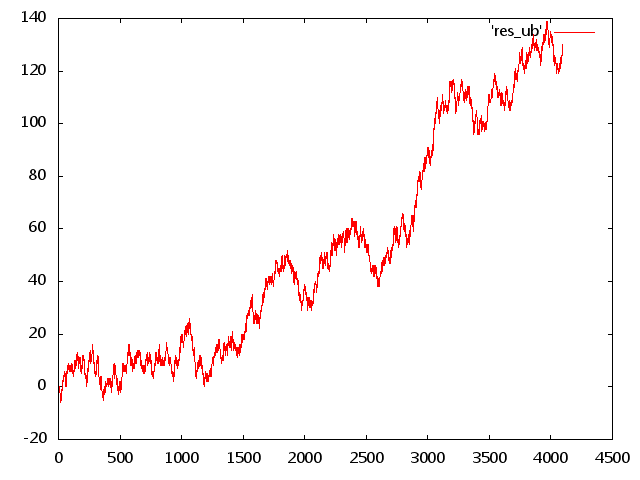
\includegraphics[width=4in]{plot_ub.png}
\end{center}
可以看出, 走了 4000 多步, 粒子离开原点的距离仅有
$140\approx2\sqrt{4000}$.

然后我们需要看一下在某个固定的时间 $t$ 抽样的 $R(t)$
满足什么样的分布. 为此需要前面写过的 \verb|count_freq|
例程, 前面解释过了. 这里只要直接调用就可以了:
\begin{verbatim}
    /* plot the frequency histogram of many random walks */
    fout = fopen("res_ub_f", "w");
    count_freq(fout, sample_r, -150.0, 150.0);
    fclose(fout);
\end{verbatim}

结果如下:
\begin{center}
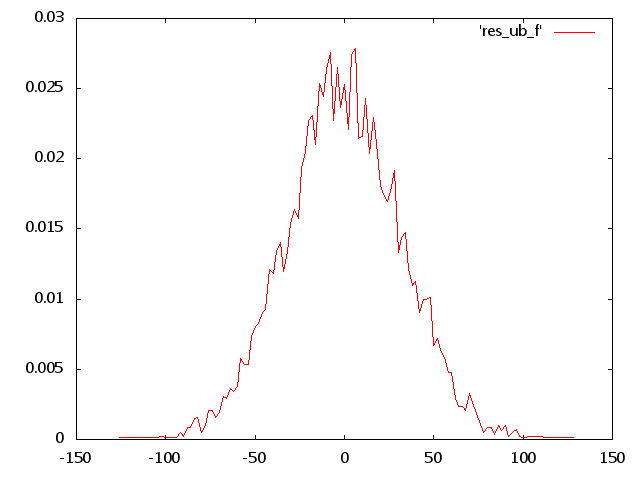
\includegraphics[width=4in]{plot_ub_f.png}
\end{center}
可以看出这分布非常接近正态分布, 这与中心极限定理的结果非常一致.

然后我们作出 $R(t)$ 的期望值 $\langle x\rangle$ 和
方均根 $\sqrt{\langle x^2\rangle-\langle x\rangle^2}$
随时间的关系:
\begin{verbatim}
    /* plot mean = \langle x\rangle and
       rms = \sqrt{\langle x^2\rangle - \langle x\rangle^2}
       versus time */
    fout = fopen("res_ub_mean", "w");
    fout_rms = fopen("res_ub_rms", "w");
    if (fout == NULL) {
        perror("fopen() res_ub_mean");
        abort();
    }
    if (fout_rms == NULL) {
        perror("fopen() res_ub_rms");
        abort();
    }
#define NSTEPS_PER_WALK    (1<<7)
    for (i = 0; i < (1<<10); i++) {
        sum = 0.0;
        sum_x2 = 0.0;
        for (j = 0; j < NSTEPS_PER_WALK; j++) {
            dist = sample_r(i);
            sum += dist;
            sum_x2 += dist * dist;
        }
        mean = sum / NSTEPS_PER_WALK;
        rms = sqrt(sum_x2 / NSTEPS_PER_WALK - mean * mean);
        fprintf(fout, "%d %.12f\n", i, mean);
        fprintf(fout_rms, "%d %.12f\n", i, rms);
    }
    fclose(fout);
    fclose(fout_rms);
\end{verbatim}
代码是非常直接的, 结果如下: 首先是 $\langle x\rangle$
\begin{center}
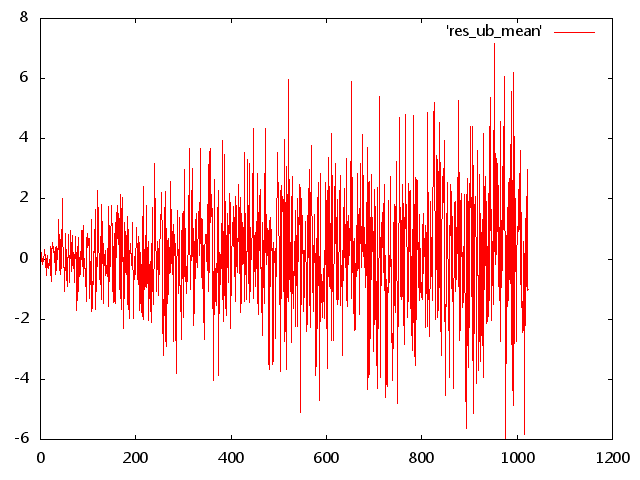
\includegraphics[width=4in]{plot_ub_mean.png}
\end{center}
可以看出 $\langle x\rangle$ 一直保持在 $y=0$ 的直线上.
注意纵坐标的刻度, 最大值在 8 远小于前面的 140.

然后是方均根:
\begin{center}
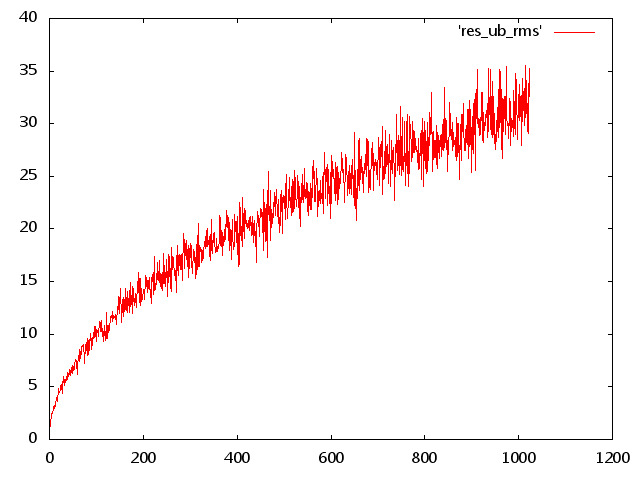
\includegraphics[width=4in]{plot_ub_rms.png}
\end{center}
前面的理论给出 (式 (\ref{rms}))
\[
{\rm RMS} = \sqrt{\int^t_0 D(\tau)\,\dd\tau}
= \sqrt{t}
\]
(因为 $D = \langle \delta r^2\rangle = 1$.)
因此理论的曲线应该是抛物线 $y=\sqrt{t}$. 这和上面
的结果非常一致. (最高点 $\sqrt{1024}=32$.)

在正弦外力场中的随机游走和上面的唯一不同就是 \verb|sample_delta_r|
要改成:
\begin{verbatim}
int sample_biased_delta_r(int t)
{
    return (rand_norm() > (0.5 +
        Param_a * sin(Param_omega*t) ) ) ? 1 : -1;
}
\end{verbatim}
其余完全一样. 代码见 \verb|biased.c|.

不同的是在这个问题中 $a$ 和 $\omega$ 都是可以任意取的
(只要 $a<0.5$). 我取了 $a=0.3$. $\omega$ 取了两个值:
$0.1$ 和 $0.01$. 先来看 $\omega=0.01$ 的结果, 这个
$\omega$ 对应的周期为 $T=\frac{2\pi}{\omega}\approx
628$. 下面是一次随机游走的图:
\begin{center}
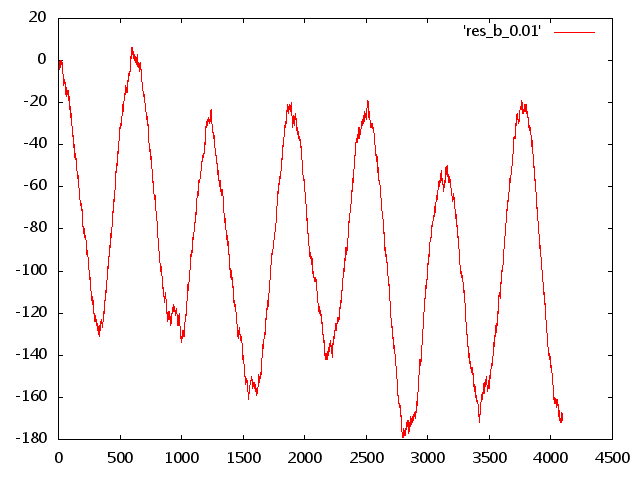
\includegraphics[width=4in]{plot_b_0.01.png}
\end{center}
可以看到振荡的效应是主导的, 带有一定随机性. 周期大概在 628
左右.

然后是固定 $t$ 时刻的 $R(t)$ 分布:
\begin{center}
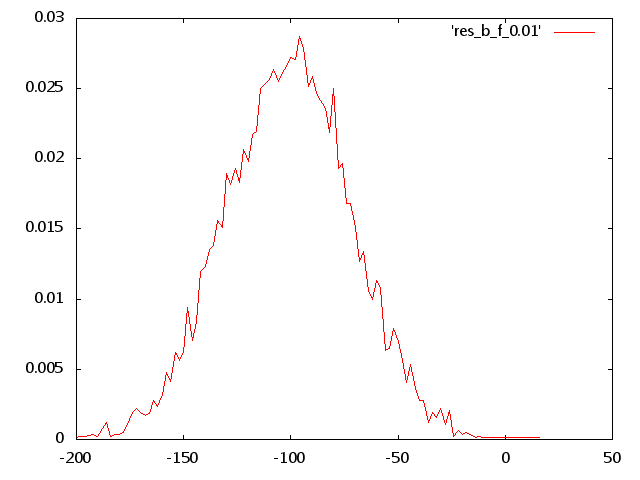
\includegraphics[width=4in]{plot_b_f_0.01.png}
\end{center}
可以看到仍然是近似的正态分布.

然后是 $\langle x\rangle(t)$:
\begin{center}
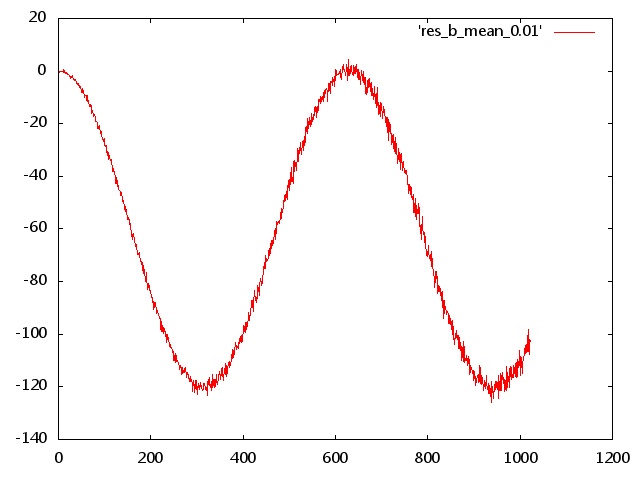
\includegraphics[width=4in]{plot_b_mean_0.01.png}
\end{center}
按照前面的理论 (\ref{mean}):
\[
\langle x\rangle = \int^t_0 \langle\delta r\rangle
(\tau)\,\dd\tau = \int^t_0 -2a\sin \omega\tau\,\dd\tau
=\frac{2a}{\omega}(\cos\omega t-1)
\]
注意到理论给出的振幅为 $\frac{2a}{\omega} = 60$ 和图上的
结果非常一致. 周期为 628 和图上的也非常一致.

最后是方均根
\begin{center}
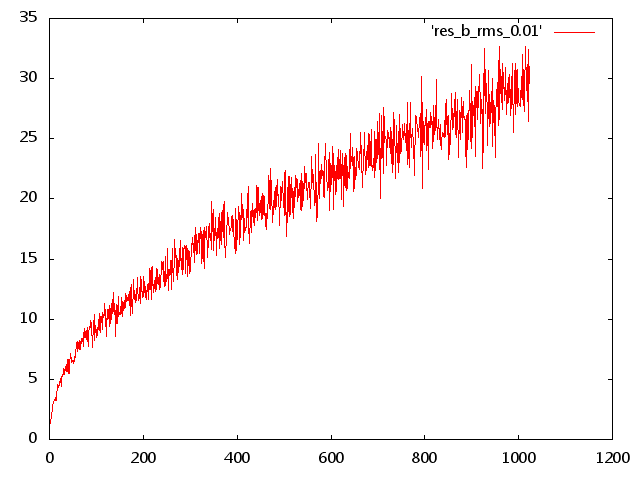
\includegraphics[width=4in]{plot_b_rms_0.01.png}
\end{center}
理论 (\ref{rms}) 给出
\[
{\rm RMS} = \sqrt{\int^t_0 \langle\delta r^2\rangle
(\tau)\,\dd\tau} = \sqrt{t}
\]
和前面经典的服从 Bernoulli 分布的随机游走的结果是一样的.
当然这里的涨落略大.

然后是 $\omega = 0.1$ 的结果, 首先是一次随机游走的 $R$-$t$ 图:
\begin{center}
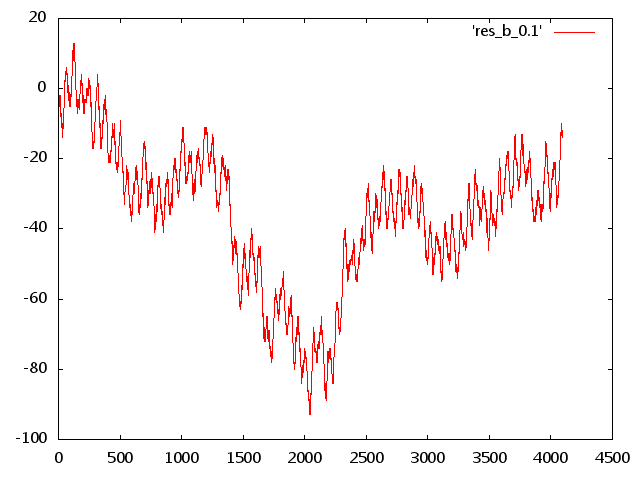
\includegraphics[width=4in]{plot_b_0.1.png}
\end{center}
这个 $\omega$ 对应的周期为 $T=\frac{2\pi}{\omega} = 63$.
和前面不同的是上面的图中随机性占了比较大的比重, 周期性较少.

然后是固定 $t$ 的 $R(t)$ 分布:
\begin{center}
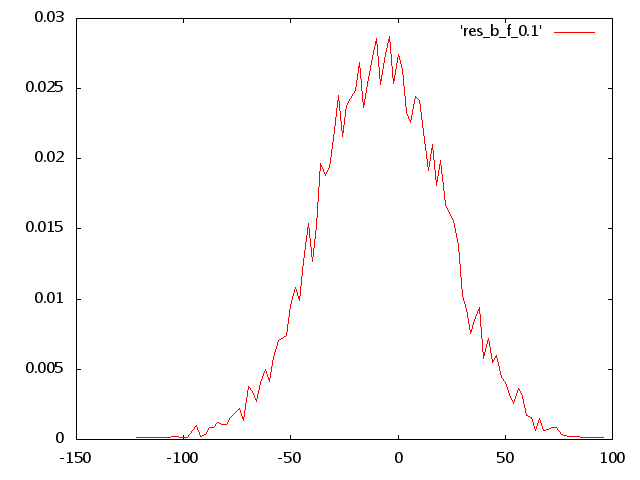
\includegraphics[width=4in]{plot_b_f_0.1.png}
\end{center}
还是正态分布.

然后是 $\langle x\rangle$:
\begin{center}
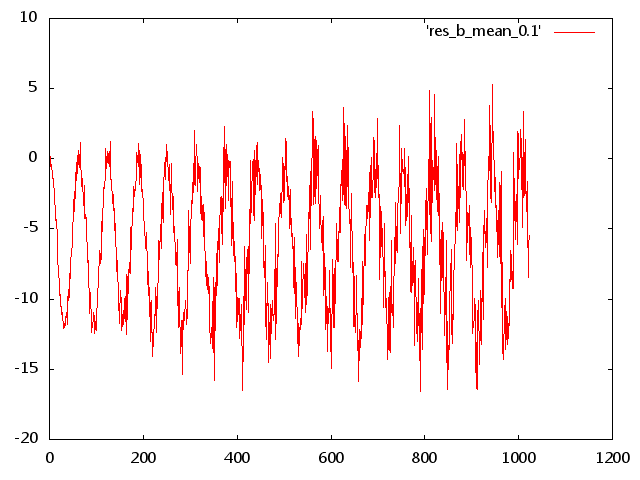
\includegraphics[width=4in]{plot_b_mean_0.1.png}
\end{center}
和前面的理论分析一致, 只不过这里涨落要比前面大.

最后是方均根:
\begin{center}
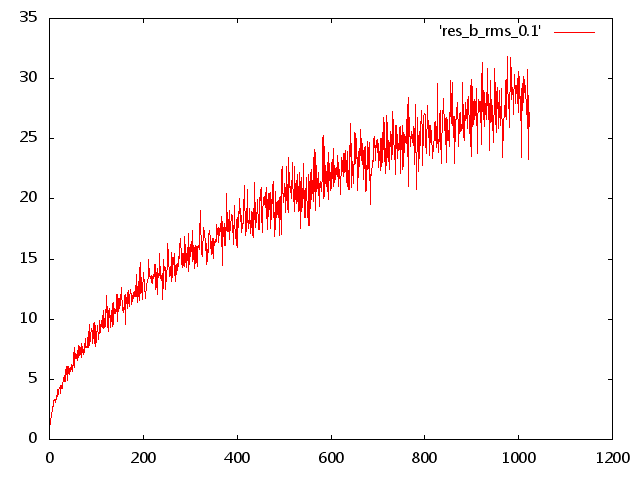
\includegraphics[width=4in]{plot_b_rms_0.1.png}
\end{center}
和前面的一样.

\end{document}